%!TEX root = ../thesis.tex
%*******************************************************************************
%****************************** Second Chapter *********************************
%*******************************************************************************
\graphicspath{{Chapter2/Figs/Vector/}{Chapter2/Figs/}}

%%%%%%%%%%%%%%%%%%%%%%%%%%%%%%%%%%%%%%%%%%%%%%%%%%%%%%%%%%%%%%%%%%%%%%%%%%%%%%%%
% Encoding Locations
%%%%%%%%%%%%%%%%%%%%%%%%%%%%%%%%%%%%%%%%%%%%%%%%%%%%%%%%%%%%%%%%%%%%%%%%%%%%%%%%
% - In what way can locations be represented to be universally interpretable?
%
\chapter{Encoding Locations}
\section{Introduction}
The term 'geospatial' denotes "relating to the relative position of things on earth's surface". This chapter concretizes the definition of a location. The way of storing and matching locations, and solving the complementary problems will be discussed.

%%%%%%%%%%%%%%%%%%%%%%%%%%%%%%%%%%%%%%%%%%%%%%%%%%%%%%%%%%%%%%%%%%%%%%%%%%%%%%%%
% A Brief History Of Geographic Locations
%%%%%%%%%%%%%%%%%%%%%%%%%%%%%%%%%%%%%%%%%%%%%%%%%%%%%%%%%%%%%%%%%%%%%%%%%%%%%%%%
% - How did the history of navigation evolve?
% - Who and what played a big role in navigation?
%
\section{A Brief History Of Geographic Locations}
A location is roughly described as a place or position. Throughout history, various navigational techniques and tools like the sextant, nautical chart and mariner's compass were used, measuring the altitude of the North Star to determine the latitude $\phi$, in conjunction with a chronometer to determine the longitude $\lambda$ of a location on the earth's surface. The combination of coordinates is a distinct encoding of a location.

\begin{figure}[htbp!]
	\centering
	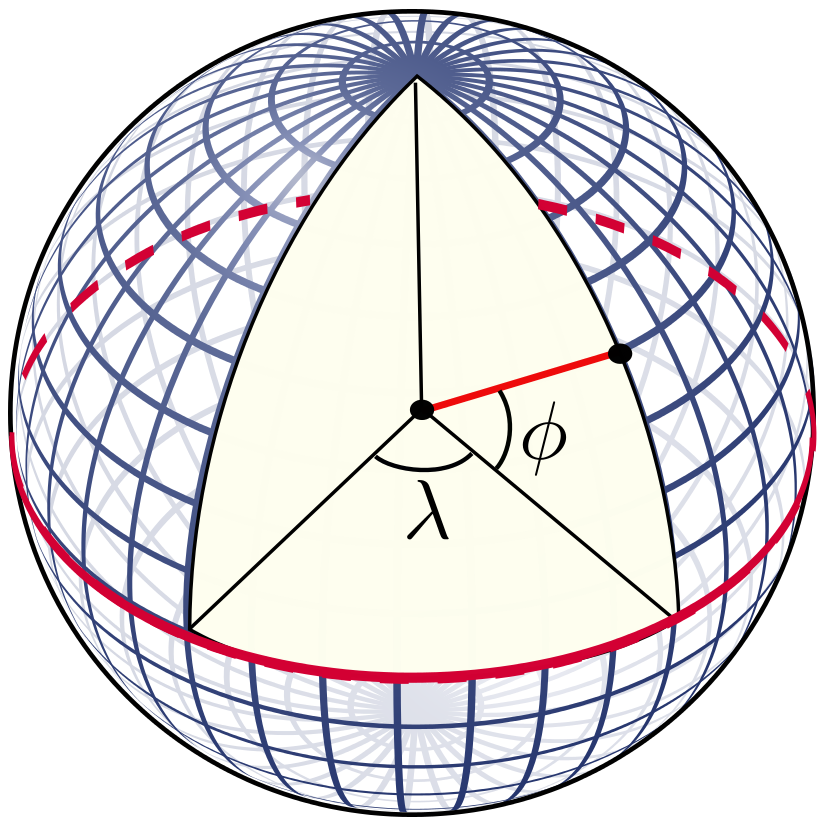
\includegraphics[width=.2\textwidth]{LatLngSphere}
	\caption[Latitude Longitude on a Sphere]{A perspective view of the Earth showing how latitude and longitude are defined on a spherical model.}
	\label{fig:latlngsphere}
\end{figure}

Today, navigation relies on satellites that are capable of providing information to determine a location with a precision of 9 meters. Hybrid methods using cell towers, Wi-Fi Location Services, and the new Galileo global navigation satellite system, provide tracking with a precision down to the meter range. These locations are ordinarily communicated using the same established latitude and longitude encoding. For a human being, it is not practical to exchange day-to-day locations as geographical coordinates. For that, addresses much more suitable, but can be ambiguous, imprecise, and inconsistent in format. Addresses commonly make use of postal code systems, which have reliably been assigned to geographical areas with the purpose of sorting mail. Although even today, there are countries that do not have a postal code system. This forces the legacy system to support addresses for the fixed pricing functionality as well. In contrast to the geographic coordinate system, postal codes describe streets and areas of varying shapes and sizes. A location being roughly described as a place or position, can be decomposed as an abstract term to describe physical or imaginary areas with varying radiuses and shapes. You could prepend 'the location of' to the following terms as an example: America, the birthplace of Socrates, Wall Street, the center of the universe, the Laryngeal Nerve of the Giraffe, churches in the Netherlands. The final example presents the main challenge of this project, how to communicate the location of a collection with points or areas of differing shapes and sizes that may overlap?

%%%%%%%%%%%%%%%%%%%%%%%%%%%%%%%%%%%%%%%%%%%%%%%%%%%%%%%%%%%%%%%%%%%%%%%%%%%%%%%%
% Requisites of Location types
%%%%%%%%%%%%%%%%%%%%%%%%%%%%%%%%%%%%%%%%%%%%%%%%%%%%%%%%%%%%%%%%%%%%%%%%%%%%%%%%
% - What do we need to describe our type of locations?
% - What do we not need?
% - Which location types matter for this project?
% - What are the main differences between postal systems used around the globe?
% - Can postal codes be abstracted to geospatial data while retaining the same
%   usefulness in the system?
%
\section{Requisite Location Types}
While setting up a backlog for a project, a shared knowledge about the terminology used in the issues must be achieved in order to collaborate effectively. Words or symbols do not have an absolute meaning, and ambiguity of abstract linguistic terms should be elucidated. In section 3.2.1 of Appendix \ref{appendix:pregame}, an agreement was made on what the terms "area" and "point" meant. The MySQL documentation notes that "The term most commonly used is geometry, defined as a point or an aggregate of points representing anything in the world that has a location." in \cite{MySQL-Spat}. During the process of implementing TPS, the definitions of a location have been refined to represent a common and useful understanding.

\subsection{The Point}
A point is a unique place expressed as a distinct coordinate pair. An address in the legacy system could be translated to a point. For example, the address that is tied to Schiphol arrival is: Aankomstpassage, 1118 AX Schiphol Centrum.
The point that encodes this location is (52.308891, 4.760900). This location is contained in the set of all possible points on Earth, which could be expressed using set builder notation:
\[P = \{(\phi,\lambda) \in \mathbb{R}^2 | -90 < \phi < 90, -180 < \lambda < 180 \}\]
\[(52.308891, 4.760900) \in P\]
A point itself can not be used to match whether another point is contained within it, because the probability of a match is infinitesimal. Only when decimals were disregarded to decrease the precision of a point, or if the origin of the point would be provided by some service, the distinct point would be a viable option to match locations.

\subsection{The Area}
An area is a set of points points with an infinite granularity. This definition allows for an area to have holes inside them, consist of other locations and contain other locations, and be infinitely precise. The most useful property of this area is to check whether a point is contained within the area, or which areas contain a given point. For this to be the case, the points must be packed together to form a shape. This definition, however conceptually valuable, will not be of much practical use. For example, $P$ is an infinitely long set of coordinates, an area that represents the earths surface. If $\phi$ ranged between 0 and 90, the set should describe all points located in the northern hemisphere, but would still be infinitely long. Checking whether a given point is contained by checking an infinite amount of real number pairs will take an infinite amount of time in the worst case scenario. Such an area can be described as a subset of all points:
\[a_1 \subseteq P \]
The set of all possible areas can be defined by the power set of P:
\[A = \mathcal{P}(P)\]
such that an arbitrary subset of points, called an area, is an element of all possible areas A:
\[a \in A\]
At the equator, 1 degree is 111320m, so 0.000001 degrees is
around 11cm. Six decimal places will be sufficient for location matching for this application. But even when reducing coordinates to having six decimal places, it would be impractical. For this reason, it is more realistic to only describe the rough edges of an area using a polygon shape. Polygon geometry is widely supported by database systems. Instead of checking for a single point in a non-terminating iteration over all points in an area, a mathematical calculations could be used to check whether a unique point is contained within the polygon.

\subsection{Postal Codes, Addresses, and Polygons}
All postal codes that start with a ten describe the city of Amsterdam, the entire area of Amsterdam can be drawn as a big polygon containing all the postal codes that start with a ten.

\begin{figure}[H]
	\centering
	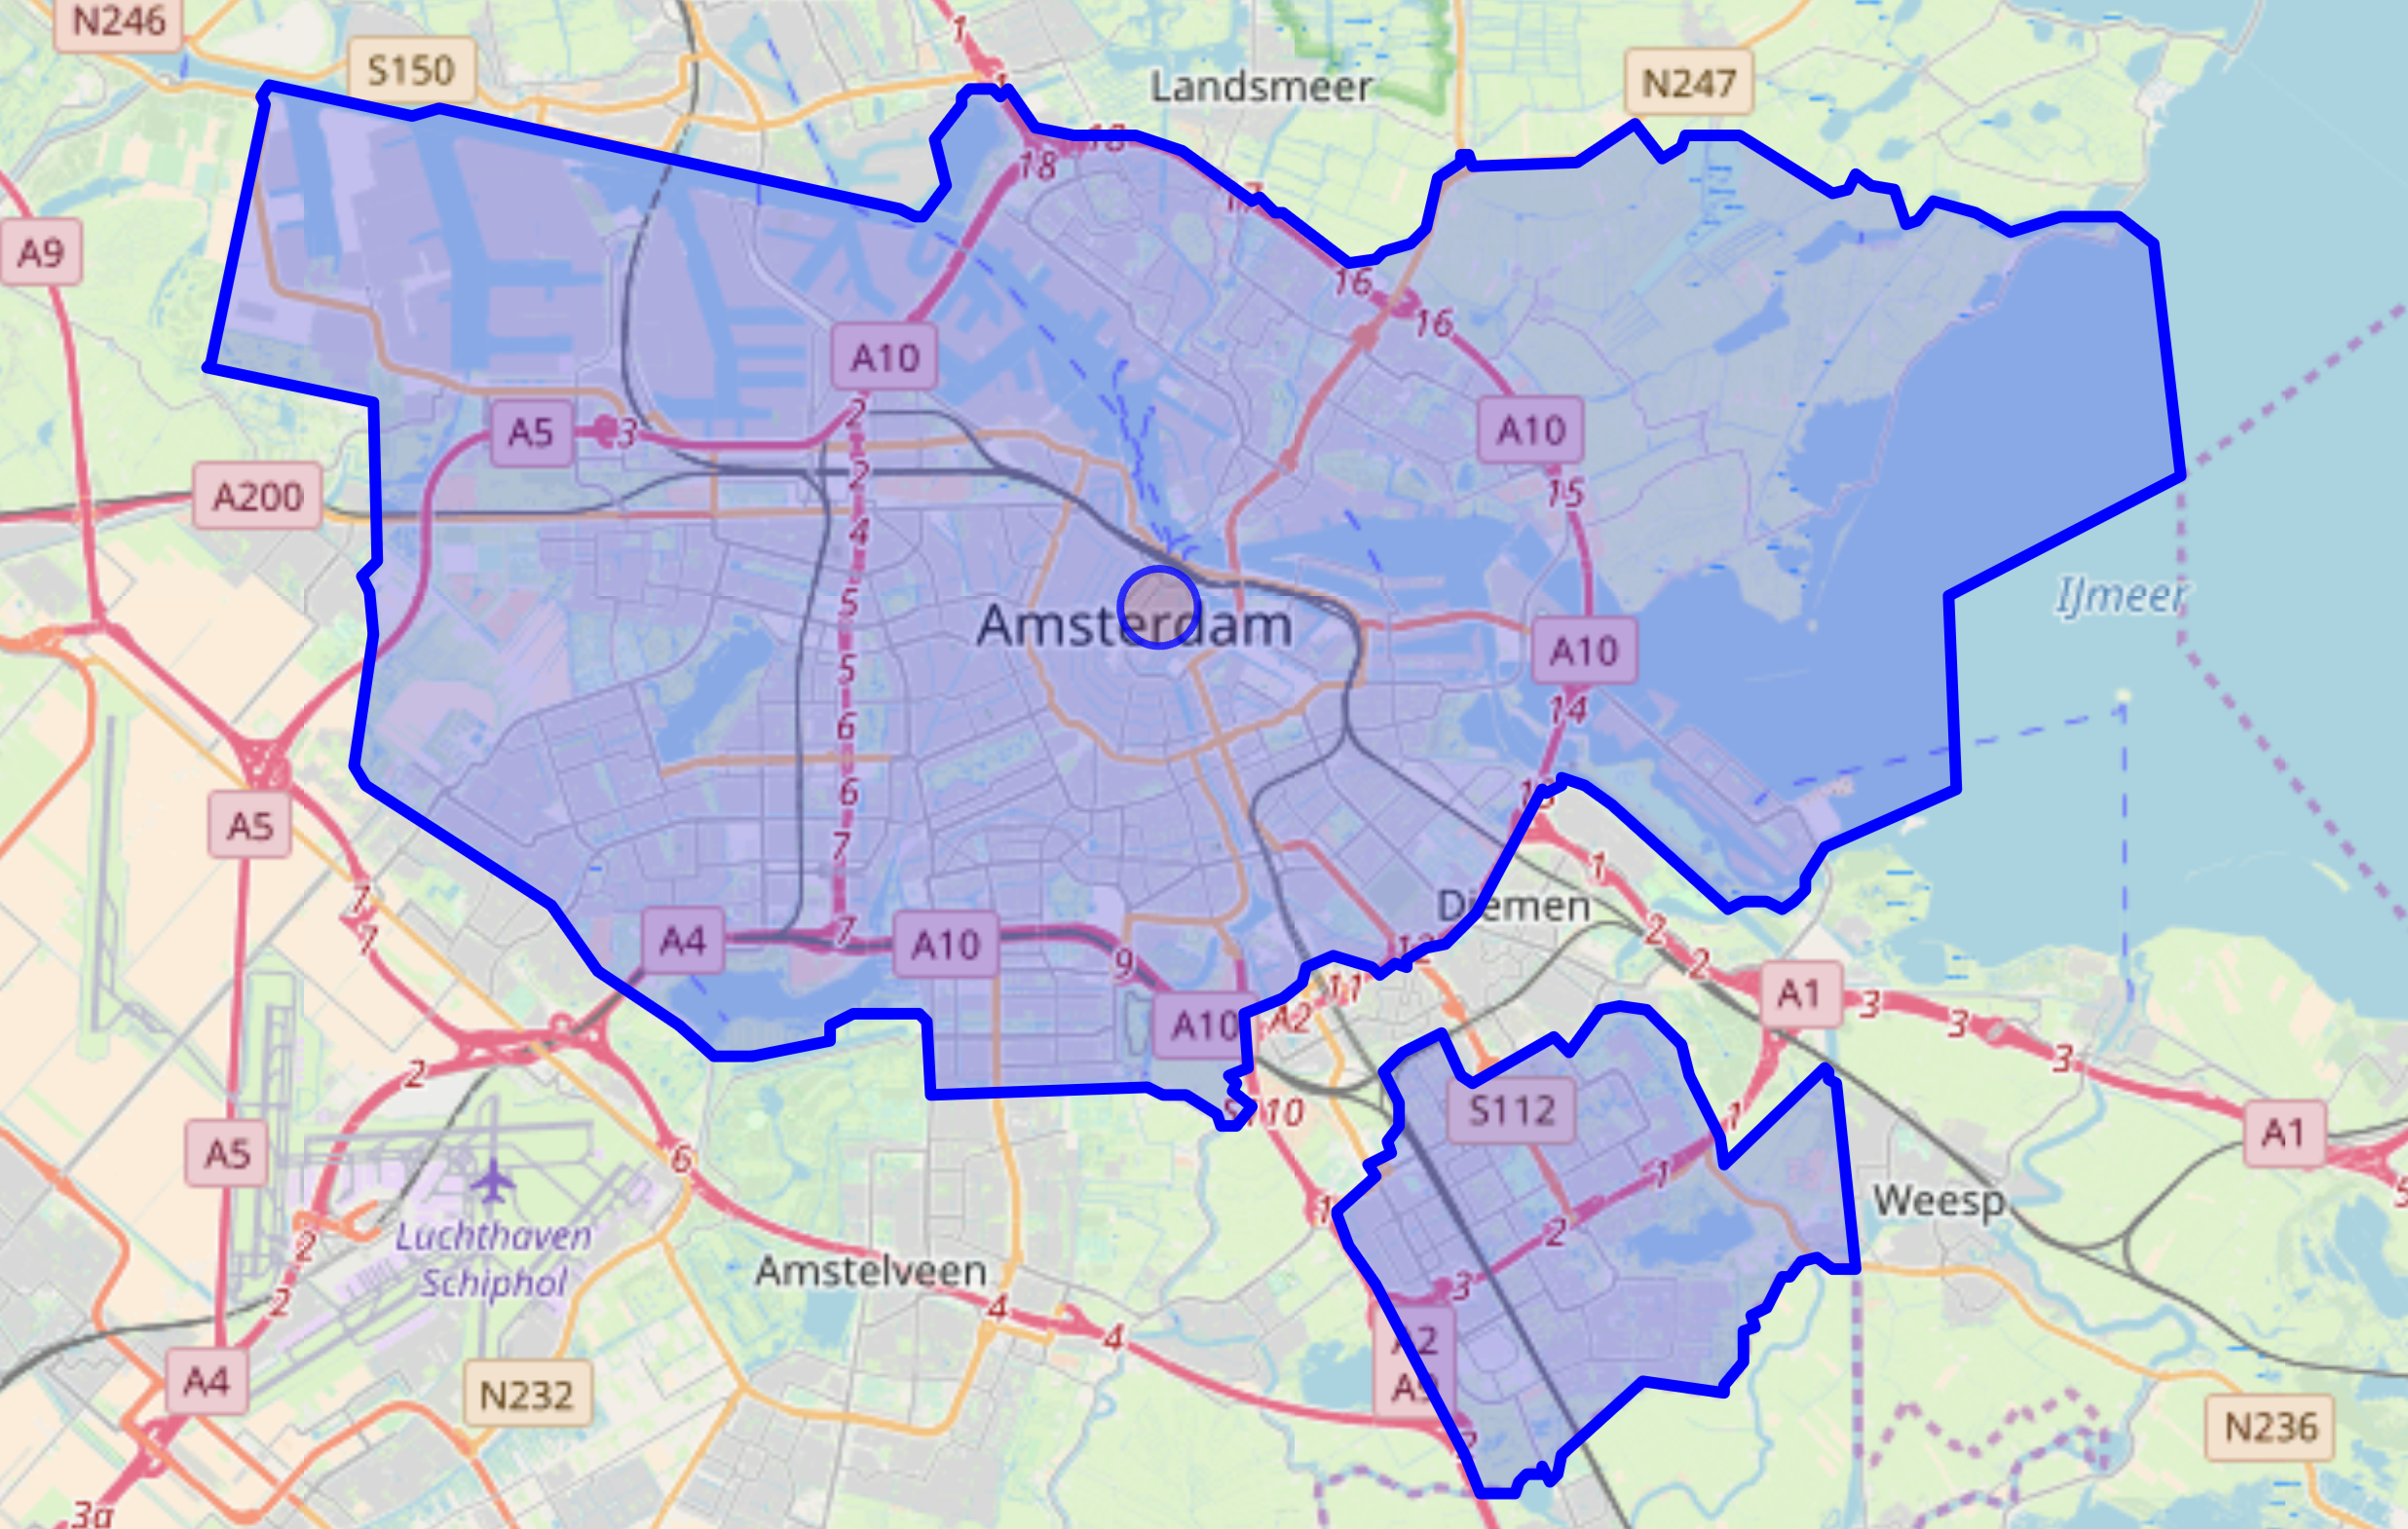
\includegraphics[width=.8\textwidth]{Amsterdam}
	\caption[Amsterdam Drawn Polygon]{Amsterdam - A single area comprised of multiple locations.}
	\label{fig:Amsterdam}
\end{figure}

In reverse, this procedure would not work. If a polygon was drawn cutting Amsterdam in half diagonally, a single postal code pattern would never be flexible or precise enough to be able to describe the boundaries of the polygon. One big taxi company making use of taxiID's legacy system is located in the United Arab Emirates. This company would not be able to convert anything at all, because the United Arab Emirates does not have a postal code system to begin with. Regardless, addresses and postal code systems do not provide universally interpretable and precise encodings of locations, especially for the locations that matter for this project: points and areas. They can be ambiguous, imprecise, and nonuniform. In the United Arab Emirates, addresses can still be utilized, even though it is harder to ensure that two addresses match. Street numbers, punctuation, formats and special characters, may cause the matching process to fail. In contrast, polygons would provide unique and precise location definition that is uniform and universal. When moving to other encoding techniques, this usefulness must be preserved.

\subsection{Requirements for Location Matching}
If the following statements are true for a given location encoding using the definitions of the Point and Area, the location encoding is useful and able to operate independently from the postal code and address systems.

\begin{table}[htbp!]
	\centering
	\begin{tabular}{l|l}
		\toprule
		Nr & Description \\
		\midrule
		1. & Every location is stored in a database as a single entity \\
		\hline
		2. & \makecell[l]{Locations can consist of multiple locations \\
			(see figure \ref{fig:Amsterdam})} \\
		\hline
		3. & \makecell[l]{A predicate of whether a location is \\
			fully contained within a location is achievable} \\
		\hline
		4. & \makecell[l]{A method of finding all locations containing \\
			a single location can be used} \\
		\hline
		5. & \makecell[l]{A method of determining precedence of location in case \\
			of overlap must always yield one result, and discard all others} \\
		\hline
		6. & \makecell[l]{Locations must be importable from external sources} \\
		\bottomrule
	\end{tabular}
	\caption[Location Matching Requirements]{Location matching requirements.}
	\label{tab:location-matching-requirements}
\end{table}

%%%%%%%%%%%%%%%%%%%%%%%%%%%%%%%%%%%%%%%%%%%%%%%%%%%%%%%%%%%%%%%%%%%%%%%%%%%%%%%%
% Literature review
%%%%%%%%%%%%%%%%%%%%%%%%%%%%%%%%%%%%%%%%%%%%%%%%%%%%%%%%%%%%%%%%%%%%%%%%%%%%%%%%
% - Storing location data
% - Querying location data
% - Intersecting
% - Research different countries
% - 3 words, gps, geospatial
%
\section{Literature Review}
In \cite{w3w}, CEO Chris Cheldrick explains how locations can be communicated more effectively by describing a three by three meter areas using three words that are assigned to the area. The system aims to solve the problem of ambiguity in address or postal code systems. The what3words API offers functionalities that can find what3word geocodings near a specified latitude and longitude location. The system is able to find results within a clamped area, as documented in \cite{w3w-api}, effectively acting like a spherical circle with a given radius in which points can be contained. In the paper \cite{spatial-data-types} Markus elaborates on the distinction between structure-based spatial data and point sets, stating that: "Structure-based spatial data types have prevailed and form the basis of a large number of data models and query languages for spatial data". He elaborates on distinctions of operations and predicates between different spatial data models in \cite{geometry}. Operations such as point-in-polygon test and intersection are categorized as spatial modeling. Regular spatial database systems support a basic Geometry hierarchy of Points, Polygons, MultiPoint and MultiPolygon Classes, as described in the OGC~\cite{SFA} and ISO 19125~\cite{ISO-19125} standard. MySQL, PostgreSQL, MariaDB and other systems having distinct implementations adhere to the OGC standard. Some other databases like MongoDB adopt the GeoJSON standard \cite{MongoDB-GeoJSON}, providing similar operations and data types. Xiang et al proposed conventional flattened R-Tree indexing for the less mature MongoDB spatial system \cite{MongoDB-implementation}. The built in Geohashing method is typically used to index points and centroids, having the possibility to inaccuracies and missing data. Locations should be importable in geography formats. Holmberg extracts data from OpenStreetMap as shape files, see \cite[Chapter~6]{openstreetmap}. He uses two sources: \url{https://www.openstreetmap.org} and \url{http://download.geofabrik.de} see \cite[Chapter~7.3]{openstreetmap}. The latter is used to obtain data for whole countries. OpenStreetMap offers a downloadable dataset at \url{https://planet.openstreetmap.org} from which geographic data can be exported.
The OSM Nominatim Usage policy states that no heavy usage is allowed, that bulk geocoding is restricted, that auto-complete is not supported, and that attribution must be displayed \cite{OSM-policy}.

%%%%%%%%%%%%%%%%%%%%%%%%%%%%%%%%%%%%%%%%%%%%%%%%%%%%%%%%%%%%%%%%%%%%%%%%%%%%%%%%
% Database Prerequisites
%%%%%%%%%%%%%%%%%%%%%%%%%%%%%%%%%%%%%%%%%%%%%%%%%%%%%%%%%%%%%%%%%%%%%%%%%%%%%%%%
% - Which Database Management Systems (DBMS) cover the location storage use
%   cases for this project?
%
\section{Database Prerequisites}
The database that is used must be able to aggregate all polygons containing a given point. Conversely, it must be able to aggregate all points that are contained within a given polygon. The scenario presented in image \ref{fig:square} should at least be replicable.

\begin{figure}[htbp!]
	\centering
	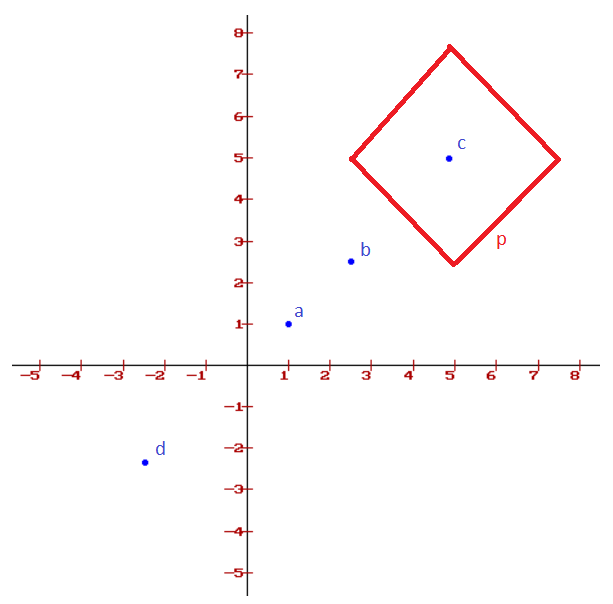
\includegraphics[width=.5\textwidth]{Square}
	\caption[Square Containing One Point]{Four Points, one Polygon p containing Point c.}
	\label{fig:square}
\end{figure}

This overly simple example provides proof that a minimal requirement is satisfied, so that a list of candidate Database Management Systems could be constructed. More complex tests have been conducted that involved different shapes, but the desired outcome remains the same. In all cases, a polygon is a list of coordinates that define a closed path, meaning that the first and last index contain identical points.

\subsection{OpenGIS Compatible databases}
MySQL's innate integrity is a good reason to opt for a full MYSQL database setup. MariaDB is a fork of MYSQL that performs better according to benchmarks, however they don’t always translate to real life situations. It’s easy to migrate from MYSQL to MariaDB, so choosing MYSQL at first could be preferable as an instance of MYSQL is already used at TaxiID. PostgreSQL offers a spatial database extender for that is OpenGIS compliant called PostGIS that adds support for geographic objects and location queries. All spatial data types inherit properties such as type and spatial reference identifier (SRID). For rigorous documentation, both PostGIS documentation \cite{PostGIS} and MYSQL documentation \cite{MySQL} could be consulted. When a generic geometry column, or point column is created, points can be inserted as shown in snippet \ref{lst:sql-insert-points}.

\begin{center}
\noindent\begin{minipage}{.85\textwidth}
\begin{lstlisting}[caption={Insert four points and one polygon in MySQL.}, label={lst:sql-insert-points}]
	START TRANSACTION;
	SET @a = ST_GeomFromText('POINT(1 1)');
	INSERT INTO point (point) VALUES (@a);
	SET @b = ST_GeomFromText('POINT(2.5 2.5)');
	INSERT INTO point (point) VALUES (@b);
	SET @c = ST_GeomFromText('POINT(5 5)');
	INSERT INTO point (point) VALUES (@c);
	SET @d = ST_GeomFromText('POINT(-2.5 -2.5)');
	INSERT INTO point (point) VALUES (@a);
	# also insert @b, @c, and @d
	COMMIT;

	START TRANSACTION;
	# First and last point should be the same
	SET @a = PolygonFromText('POLYGON((2.5 5,5 7.5,7.5 5,5 2.5,2.5 5))');
	INSERT INTO polygon (polygon) VALUES (@a);
	COMMIT;
\end{lstlisting}
\end{minipage}
\end{center}

It is evident that c is contained in p. To determine which points are contained in p, the function as seen in Snippet \ref{lst:sql-pts-in-poly} can be used, which returns the point with coordinates $[5, 5]$ as expected.

\begin{center}
\noindent\begin{minipage}{.85\textwidth}
\begin{lstlisting}[caption={Select points contained in polygon, and all polygons containing a point in MySQL.}, label={lst:sql-pts-in-poly}]
	// All points contained in polygon
	SELECT ST_ASTEXT(POINT)
	FROM POINT
	WHERE
	ST_CONTAINS(
		(
			SELECT POLYGON
			FROM POLYGON
			WHERE id = 1
		),
		POINT
	)

	// All polygons containing point
	SELECT ST_ASTEXT(POLYGON)
	FROM POLYGON, POINT
	WHERE
		POINT.id = 3 AND ST_CONTAINS(
			POLYGON.polygon,
			POINT.point
		)
\end{lstlisting}
\end{minipage}
\end{center}

A multipolygon can be inserted using triple braces, indicating a collection of polygons to be inserted as seen in Figure \ref{lst:sql-multipolygon}. The MultiPolygon class is able to support multiple polygons to be stored as a single entity. The standard provides containment predicate, and methods to distinguish larger locations from smaller ones, which could be used in precedence checks.

\begin{center}
\noindent\begin{minipage}{.85\textwidth}
\begin{lstlisting}[caption={Insert one multipolygon in MySQL.}, label={lst:sql-multipolygon}]
	START TRANSACTION;
	# First and last point should be the same
	SET @a = GeomFromText('MULTIPOLYGON(((1 1,2 2,3 3,1 1)),((5 5,6 6,8 8,5 5)))');
	INSERT INTO multipolygon (multipolygon) VALUES (@a);
	COMMIT;
\end{lstlisting}
\end{minipage}
\end{center}

\subsection{OpenGIS Incompatible databases}
MongoDB doesn’t offer OpenGIS implementations but has geospatial query operators that may provide enough functionalities for current requirements \cite{MongoDB}. The argument for choosing one over the other depends on the vast differences between SQL and NoSQL, next to performance and extensiveness of geospatial features. The setup displayed in image \ref{fig:square} is recreated in MongoDB using queries shown in snippets \ref{lst:nosql-insert-points} and \ref{lst:nosql-pts-in-poly}. Geometry datatypes can be inserted as objects having a type and coordinates property. A polygon can be inserted in the same manner, having multiple points as a list instead of a single point.

\begin{center}
\noindent\begin{minipage}{.85\textwidth}
\begin{lstlisting}[caption={Insert four points and one polygon in MongoDB.}, label={lst:nosql-insert-points}]
	db.point.insertMany([
		{ shape: { type: "Point", coordinates: [1, 1] } },
		{ shape: { type: "Point", coordinates: [2.5, 2.5] } },
		{ shape: { type: "Point", coordinates: [5, 5] } },
		{ shape: { type: "Point", coordinates: [-2.5, -2.5] } },
	])

	db.polygon.insert({
		shape: {
			type: "Polygon",
			coordinates: [ [2.5, 5], [5, 7.5], [7.5, 5], [5, 2.5], [2.5, 5] ]
		}
	})

	db.point.createIndex({ 'shape': '2dsphere' })
	db.polygon.createIndex({ 'shape': '2dsphere' })
\end{lstlisting}
\end{minipage}
\end{center}

A method named $\$geoWithin$ can be used to return points that are contained within the polygon. Conversely, all polygons that contain a certain point can be queried using the $\$geoIntersects$ method as seen in \ref{lst:nosql-pts-in-poly}.

\begin{center}
\noindent\begin{minipage}{.85\textwidth}
\begin{lstlisting}[caption={Select points contained in polygon, and all polygons containing a point in MongoDB.}, label={lst:nosql-pts-in-poly}]

	// All points contained in a polygon
	db.point.find({
		shape: {
			$geoWithin: {
				$polygon: [
					[2.5, 5],
					[5, 7.5],
					[7.5, 5],
					[5, 2.5],
					[2.5, 5]
				]
			}
		}
	})

	// All polygons containing a point
	db.polygon.find({
		shape: {
			$geoIntersects: {
				$geometry: {
					type: "Point",
					coordinates: [5, 5]
				}
			}
		}
	})
\end{lstlisting}
\end{minipage}
\end{center}

In MongoDB, a multipolygon can be inserted using extra pairs of braces, as shown in \ref{lst:nosql-multipolygon}. Any predicate will fail if the type is defined as 'Polygon', but a MultiPolygon is stored in the coordinates property or vice versa. Therefore, it is important to manage the type property as more polygons are to be stored at once.

\begin{center}
\noindent\begin{minipage}{.85\textwidth}
\begin{lstlisting}[caption={Insert one multipolygon in MongoDB.}, label={lst:nosql-multipolygon}]
	db.polygon.insert({
		shape: {
			type: "MultiPolygon",
			coordinates: [
				[ [ [2.5, 5], [5, 7.5], [7.5, 5], [5, 2.5], [2.5, 5] ] ],
				[ [ [2.5, 5], [5, 7.5], [7.5, 5], [5, 2.5], [2.5, 5] ] ]
			]
		}
	})
\end{lstlisting}
\end{minipage}
\end{center}

\section{Overlapping Locations}
If the destination is contained in several polygons associated with multiple rules, which rule should then be used to calculate the final price? A database will just pick the first result when the results are limited to one. Several solutions have been proposed to solve this problem:

\begin{enumerate}
	\item Using the location with the shortest distance from its centroid to the destination.
	\item Picking the location with the smallest area.
	\item Picking the location that has the rule with the lowest price.
	\item Picking the rule that as the highest precedence assigned by the user.
	\item A combination of these proposals.
\end{enumerate}

All listed solutions will work in the databases listed in this chapter, as the centroid and area can be calculated in OGC and GeoJSON databases.

%%%%%%%%%%%%%%%%%%%%%%%%%%%%%%%%%%%%%%%%%%%%%%%%%%%%%%%%%%%%%%%%%%%%%%%%%%%%%%%%
% Premise
%%%%%%%%%%%%%%%%%%%%%%%%%%%%%%%%%%%%%%%%%%%%%%%%%%%%%%%%%%%%%%%%%%%%%%%%%%%%%%%%
%
\section{Conclusion on Encoding Locations}
\[\textit{"Which location encoding is sufficient for this system to be operational?"}\] \hfill

Addresses and postal codes can be translated to geometric datatypes such as Points, Polygons and MultiPolygons. Geometry based locations can be visualized, and thus interpreted regardless of the country in which a location resides. Matching is done through the OpenGIS or GeoJSON API, by writing geospatial queries depending on the selected candidate database system. Selected candidate database systems are systems that adhere to the OpenGIS or GeoJSON standard, yielding many possibilities, of which MySQL and MongoDB have been proven to be workable. The problem of overlapping locations, can be solved using complex and straight forward approaches, thus proving this location encoding to be sufficient for this system to be operational.